%# -*- coding: utf-8-unix -*-
%%==================================================
%% chapter02.tex
%%==================================================

%\bibliographystyle{sjtu2}%[此处用于每章都生产参考文献]
\chapter{相关理论、技术和工具研究}
\label{chap:web_dev}
软件工程是研究和应用如何以系统性的、规范化的、可定量的过程化方法去开发和维护软件\supercite{radatz1990ieee},以及如何把经过时间考验而证明正确的管理技术和当前能够得到的最好的技术方法结合起来的学科。它涉及到程序设计语言、数据库、软件开发工具、系统平台、标准、设计模式等方面。所以本课题首先学习了软件开发尤其是WEB开发的相关理论,调研、比较并选择了一些主流的WEB开发技术和高效的WEB开发工具,以期能够用快速、高效、低成本地完成系统的开发。
\section{设计理论}
本系统在开发速度、可重用性、UI/UE、响应式、实时性等方面具有较高的要求,这就意味着传统的瀑布式开发、CSS+HTML、ajax请求等WEB开发理论不能达到本系统的要求。本章学习的理论可以给开发明确可行性、指明开发的方向、提高效率、减少重复造轮子,从而保证系统的顺利实现。
\subsection{敏捷开发}
敏捷开发有很多种,它们的具体名称、理念、过程、术语都不尽相同,相对于“非敏捷”,更强调程序员团队与业务专家之间的紧密协作、面对面的沟通(认为比书面的文档更有效)、频繁交付新的软件版本、紧凑而自我组织型的团队、能够很好地适应需求变化的代码编写和团队组织方法,也更注重软件开发過程中人的作用。\supercite{beck2013agile}

Clarity是一家创业公司,业务需求变化迅速,人员结构比较精简,因此更加适合用敏捷开发。本系统的软件开发团队由3个人组成,每天早晨与需求方即公司CEO和硬件开发团队进行视频通话来总结前一天的开发进度和确定当天的开发任务,不断地在测试服务器部署新特性(feature)版本和在生产服务器部署热修复(hotfix)版本,每个特性完成后再正式发布(release)到生产服务器上,团队成员吃住同行、分工灵活,每个人都能独当一面。

\subsection{响应式设计}
响应式设计是一种WEB设计方法,旨在构建出可以提供跨设备的(从桌面电脑到移动设备)拥有最佳的视觉和交互体验的网站,方便用户使用最少的缩放、平移和滚动操作来阅读和浏览。\supercite{marcotte2013responsive}为自动适应浏览者的设备环境,响应式网站使用流式的基于比例的网格布局,弹性的图片和CSS3 media queries\footnote{没有正式的中文译名,直译为媒体查询,是CSS中@media规则的扩展}做到了以下几点:
\begin{description}
  \item[流式网格] 流式网格要求页面元素按照如百分比之类的相对单位来缩放而不是传统的如像素或点的绝对单位;
  \item[弹性图片] 为防止图片显示时超出容器范围,弹性图片也按照相对单位来缩放;
  \item[Media queries] Media queries 允许页面上的元素根据显示设备的某种属性来使用不同的样式,这里的属性主要是设备的宽度;
\end{description}

\subsection{RESTful API设计和Web Socket数据更新}
RESTful 中文名叫“具象状态传输”,全称“Representational state transfer”,它是一种包含一系列同在一个分布式网络系统中协调的组件、连接器和数据元素如何按照不同的角色进行交互的设计原则(或者叫设计风格),旨在促进系统的性能、可扩展性、简单性、可修改性、可读性、便携性和可靠性。\supercite{fielding2002principled,fielding2000architectural}相比于SOAP\footnote{Simple Object Access protocol,简单对象访问协议}和XML-RPC\footnote{XML(标准通用标记语言下的一个子集)远程方法调用}更加简单轻量,在URL处理和Payload编码上更加简洁明了。WEB应用程序最重要的REST原则是,客户端和服务器之间的交互在不同请求之间是无状态的,这就意味着服务器可以随时重启并且客户端并不关心连接的是哪台服务器,这十分适合云计算\footnote{提供动态的易扩展的虚拟化计算资源的互联网服务模式}的环境。

WebSocket 是HTML5\footnote{万维网的核心语言、标准通用标记语言下的一个应用超文本标记语言(HTML)的第五次重大修改}中一种新的通信协议\supercite{fette2011rfc},浏览器与服务器通过一个TCP\footnote{即Transmission Control Protocol 传输控制协议}连接上的全双工通信(full-duplex)进行交互,只有一开始的握手需要借助HTTP\footnote{即HyperText Transfer Protocol超文本传输协议,是互联网上应用最为广泛的一种网络协议}请求完成。它使得浏览器可以和网站进行更多更频繁更实时的交互,从而可以摒弃从前通过轮询\footnote{每隔一秒向服务器发送一个HTTP请求来获取最新数据}来获取最新数据却会给服务器带来沉重负担的方法。

Clarity如其他众多创业公司一样,选择使用云服务器来搭载自己的服务。本系统搭载在AWS云服务器上,无状态交互是可扩展性的一大保障,频繁地增删改查设备等数据资源也需要RESTful,于是设计了一套RESTful风格的API,前端和后端分别遵循API接口来实现。另一方面需要让用户能够实时地看到自己的修改以及空气质量的变化,本系统使用WebSocket来实时地更新数据,前后端分别使用收听和发送相关主题(topic)。
\subsection{Oauth}
OAuth是Open Authorization的简写,它是一个被广泛用作互联网用户使用它们的微软、Google、Facebook、Twitter等账号在不用输入它们的密码的情况下登录到第三方网站的开放授权标准。一般来讲,OAuth提供给客户端一个代表资源拥有者访问服务器资源的“安全访问授权”。它规定了资源拥有者授权第三方访问其服务器资源而无需共享它们的凭据的过程。它是专门为超文本传输协议(HTTP)设计的,本质上OAuth允许一个授权服务器在资源拥有者批准的情况下直接把访问令牌(Access Token)发送到第三方客户端,然后第三方再使用访问令牌来获取资源服务器上被保护的资源。\supercite{hardt4rfc6749}

Clarity虽然业务规模还不大,用户数量也很少,为将来接入各种社交账号登录做准备,本系统使用OAuth标准。用户登陆后除了会获得一个对应的访问令牌(Access Token)之外还有一个寿命较长的刷新令牌(Refresh Token)用来在用户短期离线后自动刷新访问令牌,而这一切除了一开始的登录都不需要用户重新输入密码,只有在用户长期离线刷新令牌也过期的情况下才需要再次登录。除了对HTTP请求做了权限验证之外,本系统对WebSocket部分也做了相应的权限验证,socket客户端连接上Socket服务器后,会先通过socket把自己的访问令牌(Access Token)发送给服务器,服务器验证后会发回一个通过验证或者未通过验证的消息,socket客户端通过收听这两个消息来知道自己是否验证成功。如果socket客户端未通过验证,就会通知前端的原本用来刷新令牌的机制去刷新访问令牌。而每次访问令牌被改变或刷新后,socket客户端都会重新发送请求认证的消息,socket服务端也会通知客户端之前的认证已经失效。

\subsection{Flux 架构模式}
Flux 是Facebook用来构建客户端WEB应用的应用架构,它利用一个单向的数据流对React\footnote{会在下一节技术架构中介绍到}的可组合的视图组件进行了有力的补充。\supercite{gackenheimer2015react}它更像是一种模式而不是一个框架,所以在这里本课题认为它属于理论而不是技术。

它与传统的MVC模型\footnote{即Model View Controller,是一种软件设计典范}不同,主要包括三部分:dispatcher、store和view,由action来触发状态(state)变化。如下图\ref{fig:flux_data_flow}所示: 所有的action会进入到dispatcher进行处理,dispatcher会产生新的state用以更新store,store选择恰当的时机更新后通过view提前注册好的消息(回调)来告诉view更新用户界面。但其实大部分情况下action由用户的操作产生,因此会有从view产生的action。

\begin{figure}[!htp]
 \centering
 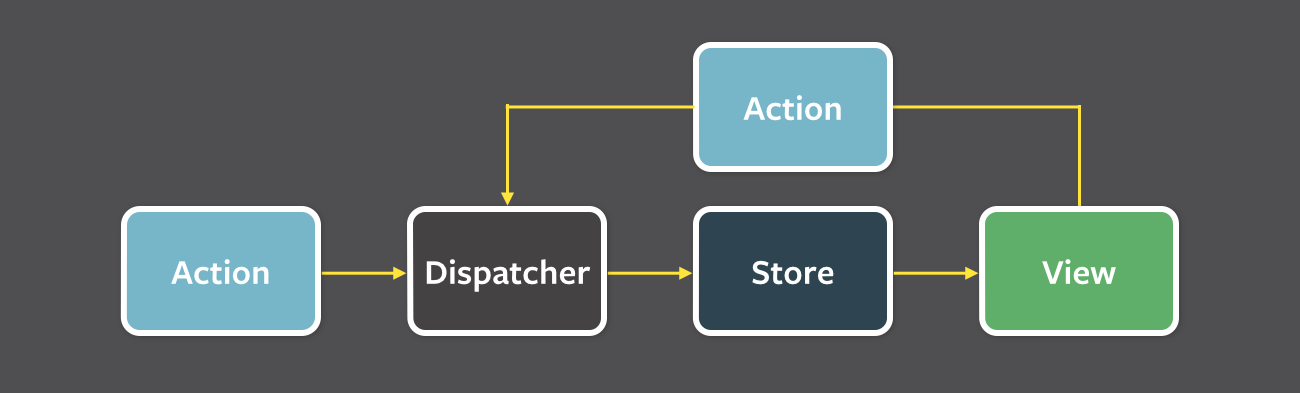
\includegraphics[width=0.9\textwidth]{flux.png}
 \bicaption[fig:flux_data_flow]{Flux 单向数据流}{Flux 单向数据流}{Fig}{Flux Unidirectional Data Flow}
\end{figure}

\subsection{SPA单页面应用和server-render服务端渲染}
单页面应用是一种只有一个网页的WEB应用,旨在给用户提供像桌面应用一样流程的用户体验\footnote{有些传统的非单页面应用,每点一个按钮,整个页面都会刷新一下,严重影响用户体验}。之所以能够做到如此,是因为所有的HTML、JavaScript和CSS文件都在最初的加载中完成\supercite{flanagan2006javascript},另有一些资源在用户交互的过程中动态的加载到页面中。整个页面在运行过程中不会重新加载,也不会突然打开一个新的页面,但地址栏中的地址会一直变化,直接输入这些地址也能够直接访问到WEB应用相应的页面。单页面应用在让用户获得流畅体验的同时,还减轻了服务端的负担,服务端更多地只是承担一个静态文件和动态资源提供者的角色。

现在中国互联网界所谓的H5移动应用\footnote{其实是一种非专业人士的误读,应该叫单页面移动应用}之所以能够流行就是得益于SPA,因为除了一开始加载比较慢,这些应用操作起来像原生移动应用一样流畅。但正所谓成也SPA,败也SPA,SPA最大的性能优点带来了它最大的性能缺点:初始加载缓慢,现在是一个节奏非常快的社会,很多人在互联网上习惯了一点链接就看到结果,缓慢加载的SPA给用户带来一种这个页面加载不出来的感觉,即使有一个旋转的加载动画也不能解决这个问题。

单页面应用初始加载缓慢导致用户体验差的核心原因是不等所有的HTML、JavaScript和CSS文件加载完成,客户端无法渲染页面,用户迟迟看不到任何信息所以才会用户体验差,于是刚刚告别了服务端渲染出来单打独斗的单页面应用又在初次加载时重新拥抱了它。使用初次加载的服务端渲染时,服务端不再是简单地、静态地提供HTML、JavaScript和CSS文件,而是先用服务器强大的计算能力替用户计算出一个能够直接被浏览器渲染的HTML,客户端先把这个结果给用户看,然后在悄悄地、缓慢地加载全部的文件。好像刚刚获得解脱的服务端又负担起了一个艰巨的负担,其实不然,\textbf{缓存}再次解决了这个问题,而且服务端缓存不像客户端缓存那么多变\footnote{客户端环境和浏览器的不同}且不可控制。

\section{技术栈}
Clarity的开发团队是一个精简且高效的年轻团队,我们选择了全栈JavaScript。从前端到后端,从业务逻辑到测试,全部使用JS,这样给我们带来了不少好处:
\begin{enumerate*}
  \item 提高了代码重用率,因为前后端可以共同使用一些代码逻辑
  \item 提高了分工灵活度,前后端的人力可以随时支援对方
  \item 提高了开发速度,因为全栈JS的生态圈很强大、包管理系统也非常省心省力
  \item 提高了代码可维护性,因为全栈JS的各种代码规范标准非常强大\ldots
\end{enumerate*}

下面就开始分前端、后端、数据库和服务器来介绍本系统将会使用到的技术栈:
\subsection{前端: Angular VS React}
目前JS的主流前端技术无外乎两个选择,Angular和React,如图\ref{fig:github_rank}所示,这两个项目在Github上排行分别是第5和第6。
\begin{figure}[!htp]
 \centering
 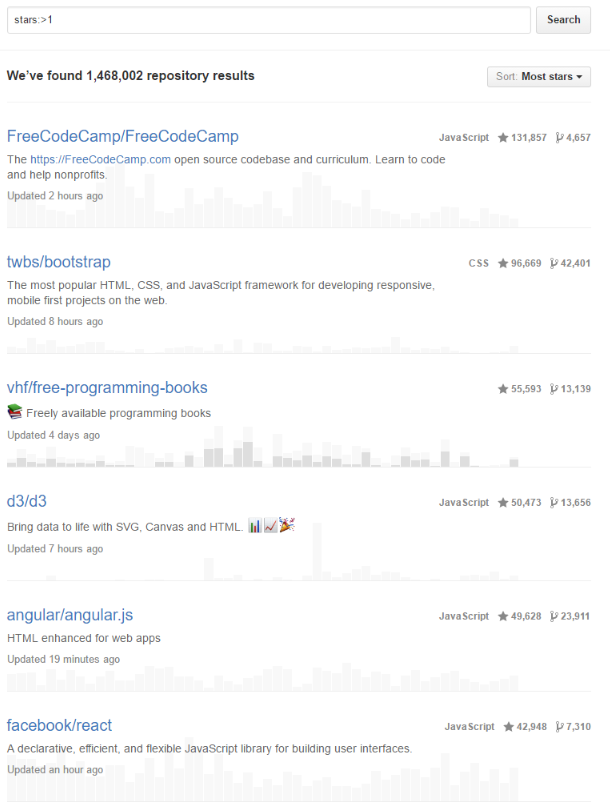
\includegraphics[width=0.9\textwidth]{github_rank.png}
 \bicaption[fig:github_rank]{Github angular和react排名情况}{Github angular和react排名情况}{Fig}{Github star ranking of angular and react}
\end{figure}
\subsubsection{Angular}
AngularJS 是一个主要由Google维护的开源WEB应用框架,另外还有一个由个人和企业组成的解决SPA\footnote{Single-page applications单页面应用}开发过程中遇到的挑战的社区参与维护。AngularJS旨在通过提供一个客户端MVC架构和MVVM\footnote{model-view-viewmodel}架构的框架来简化SPA的开发和测试,另外它还提供了许多在丰富互联网应用(Rich Internet Application)\footnote{是一种拥有很多桌面应用软件特性的WEB应用 }中被广泛使用的组件(component)directive\footnote{AngularJS中对可重用组件的定义}。AngularJS 在2010年首次发布,除了开源,它有一些创举,极大解放了前端工程师以及后端工程师的生产力:
\begin{enumerate}
  \item 使用依赖注入(dependency injection)\footnote{一种使用控制反转来处理依赖管理的软件设计模式},使得客户端也可以使用MVC,把WEB应用程序的客户端和服务端解耦合了,减轻了原本后端路由控制、页面渲染的负担,使得两边都可以被重用
  \item 使用双向绑定(two-way data binding)\footnote{视图和逻辑中的模型变量(model)互相绑定,牵一发而动全身},把DOM操作从应用程序逻辑中移除了(或者说尽量避免使用),增强了客户端程序的可测试性和性能;增强了HTML,在HTML标签中插入模型变量(model),使得开发者编写HTML时“所见既所得”。
  \item 提供了一整套构建WEB应用的过程:从UI设计,到业务逻辑,再到测试,大量的可重用组件和强大的生态圈使得开发者大量减少重复造轮子的现象
\end{enumerate}

\subsubsection{React}
ReactJS 是一个用来把视图数据渲染为HTML的开源JavaScript库,它的主要维护者是Facebook、Instagram和一个由个人开发者和企业组成的社区。React视图用以自定义HTML标签形式定义的组件(component)来渲染,这些组件可以也包含其他的组件。ReactJS 是一个年轻的库,它在2011年被首次部署,在2013年美国JS大会(JSConf US 2013)上被开源,总的来讲,ReactJS有以下几点特性是它如此成功的原因:

\begin{description}
  \item[单向数据流(One-way data flow)] 主要由前文介绍的Flux架构保证,每个组件会收到一些属性(properties)用来渲染到HTML标签中。与Angular的双向绑定不同,组件本身不可直接修改这些属性,只能通过作为属性传入的回调函数来修改,在Flux架构中,就是触发Action,这种原理被叫做“properties flow down actions flow up”。
  \item[虚拟DOM(Virtual DOM)] React构造了一个内存中的DOM缓存,统一计算每次渲染之间的差异,然后高效地对浏览器中的DOM进行差异更新,相比于Angular而言,Angular是监听每个视图模型(model)的变化,然后更新DOM中对应的部分,并没有差异更新的能力。
  \item[JSX\footnote{一种JavaScript的扩展语法,可以在JS代码中方便地引用HTML和使用HTML标签}] JSX允许React很方便地在JS代码中渲染子组件(subcomponents)。与Angular增强HTML不同,React依靠JavaScript本身的强大,更加方便地做到了一样的功能。
\end{description}

\subsubsection{综合比较与选择}
目前来说Angular是2015年的JS宠儿,而React则后来居上,其实Angular2应当能与React媲美,但是在项目研发时,Angular2离可以正式使用还有一段距离,React则已经接近正式发布。

Angular和React最大的不同在于一个是WEB框架,一个是JS库。WEB框架意味着开发一个主流的单页面WEB应用程序所需要的一切\footnote{狭义上的,当然不包括各种开发工具}Angular都提供给你了,而React崇尚小而精,它只提供了最核心的部分,其他部分都由开发者自己从社区中选择或者自己开发组合起来搭建一个WEB应用程序。如表\ref{tab:angular_vs_react}所示,Angular和React在很多方面各有不同,有些并不能分出优劣。

\begin{table}[!htpb]
  \bicaption[tab:angular_vs_react]{Angular和React的对比}{Angular和React的对比}{Table}{Comparisons between Angular and React}
  \centering
  \begin{threeparttable}[b]
    \begin{tabular}{lcr}
      \toprule
      对比 & Angular & React \\
      \midrule
      灵活度 & 一般  & 灵活多变 \\
      稳定性 & 稳定且成熟  & 接近稳定 \\
      开发速度 & 快 & 一般\\
      社区 & 强大 & 一般但快速成长 \\
      性能 & 一般 & 很高 \\
      支持Web Component\tnote{1} & 弱 & 强 \\
      视图核心语言 & HTML & JavaScript \\
      页面一致性\tnote{2} & 一般 & 强 \\
      \bottomrule
    \end{tabular}
    \begin{tablenotes}
    \item [1] React设计之初就考虑到对Web Component的支持,而Angular的发布和Web Component概念提出大概是在同一时期.
    \item [2] 在上一节的Flux介绍中提到,Angular的双向绑定可能会导致页面出现一些不一致,而程序员自己都难以定位.
    \end{tablenotes}
  \end{threeparttable}
\end{table}

本系统中版本管理模块类似传统的后台管理系统,因此选用了稳定、成熟且开发迅速的Angular;而Smart Home和Smart City模块是给用户定制的,所以选用了灵活度更大,性能更好,页面一致性更高的React。具体使用了哪些技术,在后面对模块的详细设计中会有所介绍。

\subsection{后端: ExpressJS VS KoaJS}
NodeJS是一个用来开发服务端WEB应用的开源的跨平台的运行时环境,NodeJS在运行时用Google的V8引擎\footnote{Chromium项目为Google Chrome浏览器开发的一个开源的JavaScript引擎}编译JavaScript。尽管NodeJS不是一个JavaScript框架,但它很多的基础模块都是用JavaScript写的,开发者也可以用JavaScript编写新的模块。

\subsubsection{ExpressJS}
ExpressJS是用来搭建WEB应用程序的NodeJS服务器框架,它几乎就是NodeJS标准的服务器框架。它最初的作者TJ Holowaychuk把它描述为一个由Sinatra\footnote{一个用Ruby写的免费开源WEB应用程序库,同时也是一门域专用语言(doman-specific language),特点是核心最小化,各种特性(或功能)以插件的形式来提供}启发的服务器,也就是说它是相对最小的但用插件提供了很多功能。Express作为后端部分与MongoDB数据库和AngularJS前端框架共同组成MEAD stack\footnote{一个用于构建动态网站和WEB应用的开源JavaScript捆绑包,MEAN分别指的是MongoDB, Express, Angular 和 NodeJS}。

\subsubsection{KoaJS}
KoaJS由Express原班人马倾力打造,致力于把Koa做成一个更小、更加健壮、更富有表现力的WEB框架。Koa提供了不同的generator\footnote{ES6的一种新特性,可以用一种连续的方式写异步函数},可以避免琐碎的回调函数嵌套,并极大地简化了错误处理,同时还提升了代码的可读性和健壮性,使得WEB应用开发变得得心应手。Koa的内核中没有任何事先绑定的中间件(middlewares),它只提供了一个轻量级的函数库。

\subsubsection{综合比较与选择}
从设计哲学上讲,Koa想要“修复并取代NodeJS(fix and replace node)”,而Express“补充了NodeJS(augments node)”。Koa可以被看做是NodeJS的http模块的抽象,而Express是一个NodeJS的应用框架。

\begin{table}[!htpb]
  \bicaption[tab:koa_vs_express]{Koa和Express的对比}{Koa和Express的对比}{Table}{Comparisons between Koa and Express}
  \centering
  \begin{threeparttable}[b]
    \begin{tabular}{lcc}
      \toprule
      特性/功能 & Koa & Express \\
      \midrule
      中间件内核 & √ & √ \\
      路由 & & √ \\
      模板 & & √ \\
      发送文件 &   & √ \\
      JSONP\tnote{1} &   & √ \\
      没有回调 & √ &  \\
      更好的错误处理 & √ &  \\
      不需要域 & √ &  \\
      \bottomrule
    \end{tabular}
    \begin{tablenotes}
    \item [1] JSON with Padding,是一种WEB开发者用来跨域的技术.
    \end{tablenotes}
  \end{threeparttable}
\end{table}

如表\ref{tab:koa_vs_express}所示,Koa和Express相比更加专精于HTTP的处理,且更加优秀。

本系统中版本管理模块因为技术模型比较成熟,选择了MEAN捆绑包,也就是在后端部分选择了Express。而在另外两个模块中,使用了同一个后端,且则选择了更加便于维护的Koa。与Koa相结合来使用的一些模块,在后面详细设计中会具体介绍。

\subsection{数据库: MongoDB和Mongoose}
MongoDB 是一款免费的、开源的、跨平台的、面向文档(document-oriented)的非关系型数据库。MongoDB避免了传统的基于表的关系型数据库的结构,转而使用一种类似JSON的有动态描述(schema)\footnote{数据库中用某种语言来描述的数据的结构或蓝图}的文档(documents)来存储数据,给一些特定类型的应用带来了更简便更快速的数据集成。据月度排行网站DB-engines.com统计,到2016年6月,MongoDB是世界上第四流行的数据库,并且是最流行的文档数据库。

Mongoose 是一个开源的JavaScript库,旨在为NodeJS提供优雅的MongoDB对象模型,给开发者提供了直截了当的基于描述(schema)的方法来为应用程序数据建模,包括内置的类型转换、校验、查询构建和业务逻辑Hook。
\subsection{服务器: AWS Elastic Beanstalk云服务}
AWS,全称Amazon Web Services,是亚马逊旗下的一家子公司。AWS云服务是该公司提供的一套云计算服务,这些服务组成了一个按需分配的云计算平台。AWS Elastic Beanstalk 是其中一款PaaS(平台及服务的)云服务。它允许用户创建应用程序并把他们推送到一个可定义的AWS服务集合,其中包括弹性计算云\footnote{Elastic Compute Cloud,简称EC2,可以弹性地分配计算资源,AWS最核心的服务之一},简单存储服务\footnote{Simple Storage Service,简称S3,用于文件存储,也是AWS最核心的服务之一},简单通知服务\footnote{Simple Notification Service,简称SNS}, 云监测\footnote{CloudWatch,可以实时监测EC2用户的资源利用率},自动扩展服务\footnote{autoscaling}和弹性负载均衡器\footnote{Elastic Load Balancers}。Elastic Beanstalk在简单的服务器和操作系统之上又额外提供了一层抽象,实际上用户看到的是一个预装好的操作系统和平台的组合。

\section{开发工具}
工欲善其事,必先利其器。有正确的理论指引方向和合适的技术铺平道路,还需要选择最佳的工具来加速前进。本课题调研并选择了一些最符合系统要求的工具来辅助开发,包括版本控制工具、编辑器、代码生成器、文档生成器、代码质量检测工具、编译工具、单元测试工具、持续集成工具等,本小节着重介绍了有特色的几点。
\subsection{版本控制: Git和Git-flow}
Git是一个被广泛用于软件开发和其他版本控制任务的版本控制系统(Version Control System)。它是一个强调速度、数据完整性而且支持分布式、非线性工作流的分布式版本管理系统,每一个Git工作目录(working directory)是一个带有全部历史信息和完全的版本追溯能力的完整仓库。本系统一共涉及到4个仓库,3个模块分别一个仓库,名字分别是前文提到过的balanar、azwraith和robotic。另外还有一个比较特殊的是版本管理模块的代码生成器有一个单独的仓库generator-material-app,这个会在后面详细设计中介绍到。

Git-flow是提供了一系列高级仓库操作的一个Git扩展集或者说是一个Git指令库,基于Vincent Driessen的分支模型\supercite{driessen2010successful},该模型是一个能够帮助开发者在大型项目中同时追踪数量众多的新特性(features)、热修复(hotfixes)和发布(releases)的git分支和发布策略。Git-flow管理的项目仓库中有两个主要的分支:master(生产分支)和develop(测试分支),另外还有一些辅助分支:features(新特性分支)、releases(预发布分支)和hotfixes(热修复分支)。图\ref{fig:git_flow}是Vincent在文章中给出的示例,竖直向下的轴是时间轴,横轴是不同的分支,图上的圆圈圈住的点表示发生在不同时间的不同的Commit(提交),带有箭头的线表示提交的父子关系\footnote{Git中的提交允许有多个父提交和多个子提交}。从图中可以看出这一段示例中,发生了两次多feature同时开发、一次突发hotfix和两次release。

\begin{figure}[!htp]
 \centering
 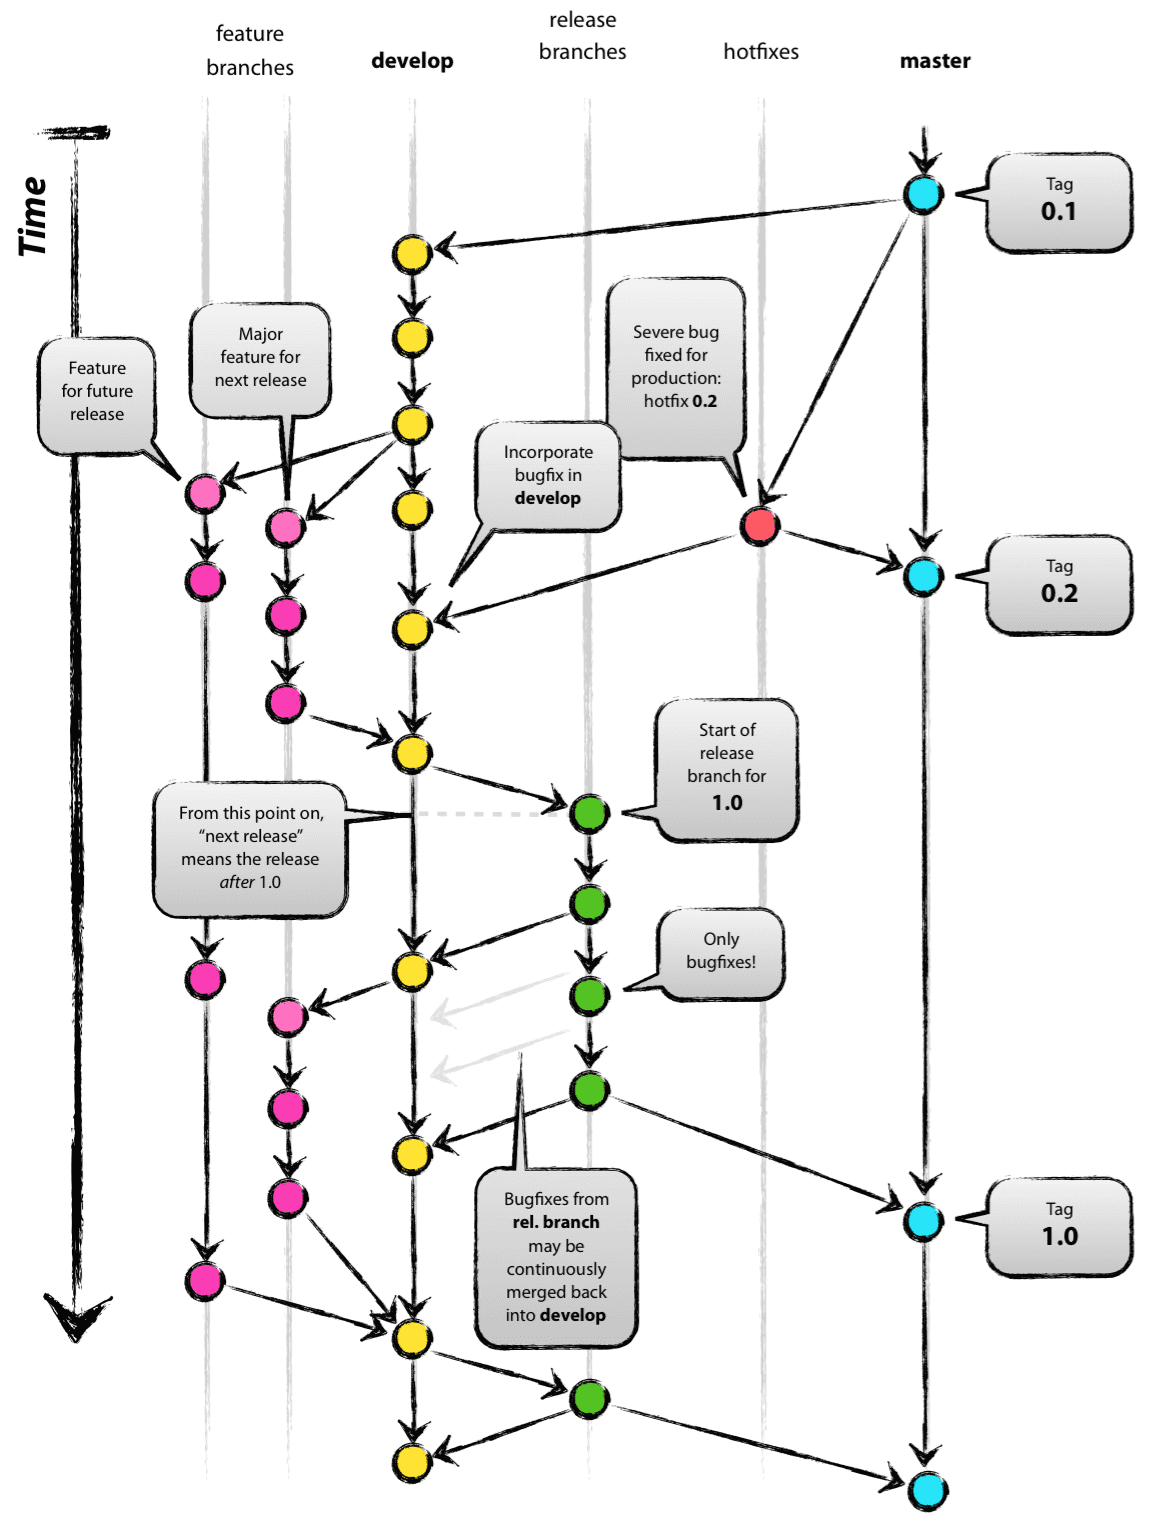
\includegraphics[width=0.9\textwidth]{gitflow.png}
 \bicaption[fig:git_flow]{Git-flow 工作机制示意图}{Git-flow 工作机制示意图}{Fig}{Git-flow working mechanism}
\end{figure}

\subsection{代码生成: Yeoman和Yeoman Generators}
Yeoman是一个开源的客户端开发工具,包括一系列帮助开发人员搭建WEB应用程序的工具和框架。Yeoman运行起来是一个命令行交互界面,工具开发人员利用它来和应用开发人员交互(或者不进行交互)获取一些信息后运行用NodeJS写的一些功能函数,如生成一个WEB应用程序的启动模板、管理依赖、运行单元测试、提供一个本地开发服务器和优化生产环境代码等。generator-material-app\footnote{\url{https://github.com/michaelkrone/generator-material-app}}是一个生成Material Design风格的MEAN应用脚手架(基本框架)的Yeoman代码生成器。

本系统在开发时,主要是版本管理模板因为是一种比较成熟的后台管理系统,使用了代码生成器来生成初始的结构和开发过程中的模块,这极大地减少了重复劳动,增加了代码可维护性,解放了开发人员的生产力。

\subsection{代码质量}
本小节介绍了一系列提高代码质量的手段和工具:代码风格指南、代码风格检查器、Git钩子机制(Git hooks)和代码审查(code review)。其中后者是前者的保障或备案。
\subsubsection{代码风格指南: John Papa和Airbnb}
风格指南(style guide)是一种编写和设计文档的标准集,不管是大众用途的还是某一个特殊领域的,比如代码编写。遵从统一的代码风格指南可以提高代码的一致性从而提高代码的可读性,一个代码风格指南一般是由一些权威的人士或者公司总结了一些最佳实践(Best practice)来编写出来的,所以能够提高代码质量,避免或减少常见错误。

当然风格指南只是一种指南,并不能保证每个开发人员至始至终遵守,人也没有精力准确地判断梅一段代码是否符合风格指南,还需要一些工具来保证代码的风格一致性。
\subsubsection{代码风格检查器: JSCS、 Jshint/ Eslint和Stylelint}
检查代码风格的一个主要工具是各种代码风格检查器,以下列出本系统中使用的各类地代码风格检查器:
\begin{itemize*}
  \item JSCS是一种针对JavaScript的语法层面的代码风格检查器
  \item Jshint是一种针对JavaScript的语法及语义层面的代码风格检查器
  \item Eslint和Jshint类似,区别是对ES6的支持比较好
  \item Stylelint是一种针对CSS的代码风格检查器
\end{itemize*}

这些代码风格检查器都通过一个简单的配置文件\textbf{.jscsrc、.jshintrc、.eslintrc、.stylelintrc},里面列有一系列的规则来自定义想要的各种代码风格。也可以通过简单的preset选项来使用某一个内置的代码风格,然后可以增加一些规则来修饰。如果在某一个单独的文件中想要突破规则也可以暂时地修改规则或者关闭规则。

有了代码质量检查器也不能保证开发人员会去使用,或者开发人员是同意使用的,但总是会有忘记和疏漏的时候。这时就需要Git hook来保障代码质量检查器的运行。
\subsubsection{Git hooks 和 Pre-commit}
Git hook是Git提供的一种钩子(hook)机制,每当你使用Git做某种操作时就会触发来执行一段脚本,比如本系统中就是用了\textbf{预提交钩子(pre-commit hook)},顾名思义就是在提交之前会执行的钩子。本系统中使用了一个开源的封装\textbf{pre-commit},配合npm脚本(scripts)只需要安装和在\textbf{package.json}中简单的配置就能在每次commit之前运行我们的代码风格检查器。

然而Git又提供了一些方法来突破钩子机制直接提交,毕竟有可能会发生恶意篡改代码风格检查器配置或者没空修复代码风格的紧急情况,所以Git hook也不是最终的保障。
\subsubsection{Code review}
一台机器可以做五十个普通人的工作,但是没有哪部机器可以完成一个伟人的工作\supercite{hubbard2015one}。最终的检查还是要靠人,代码审查(code review)是一种对软件源代码的系统性检查,目的是找出在开发阶段倍忽视的错误和提高整体的代码质量。代码质量经常能够发现一些常规的安全漏洞来提高软件的安全性,如格式字符串漏洞、竞争情况、内存泄漏和缓冲区溢出等。

本系统在开发过程中,把代码审查和前文提到的Git flow结合,每个新特性分支、热修复分支和预发布分支在合并到主要分支之前,都需要先发出一个合并请求(git上叫做pull request),然后指定团队中的一个人从客观的角度审查每一行修改,如果新增的代码或改动能让一个不够了解这个项目、这个特性的人也能看懂其意图,那么证明它的可读性和可维护性是足够高的,从而保障了主要分支代码的高质量。
